\begin{frame}[allowframebreaks]{References}
  \setbeamertemplate{bibliography item}{\insertbiblabel}
  %\nocite{*} % Insert publications even if they are not cited in the poster
  \bibliographystyle{apalike}
  \bibliography{main.bib}
\end{frame}

\begin{frame}{Motivation}
\vspace{0.5em}

\begin{figure}
\begin{columns}%
        \begin{column}{0.75\textwidth}%
            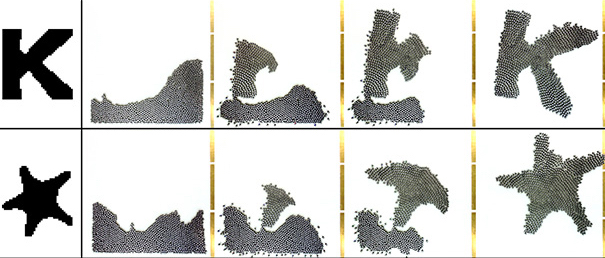
\includegraphics[width=\textwidth,right]{images/Kilobots31}
        \end{column}%
        \begin{column}{0.25\textwidth}%
            \caption{Kilobots in action \scriptsize{\cite{mike_rubenstein_kilobots31_2014}}}
        \end{column}%
    \end{columns}
\end{figure}

\vspace{1.5em}
\begin{figure}
\begin{columns}%
        \begin{column}{0.75\textwidth}%
            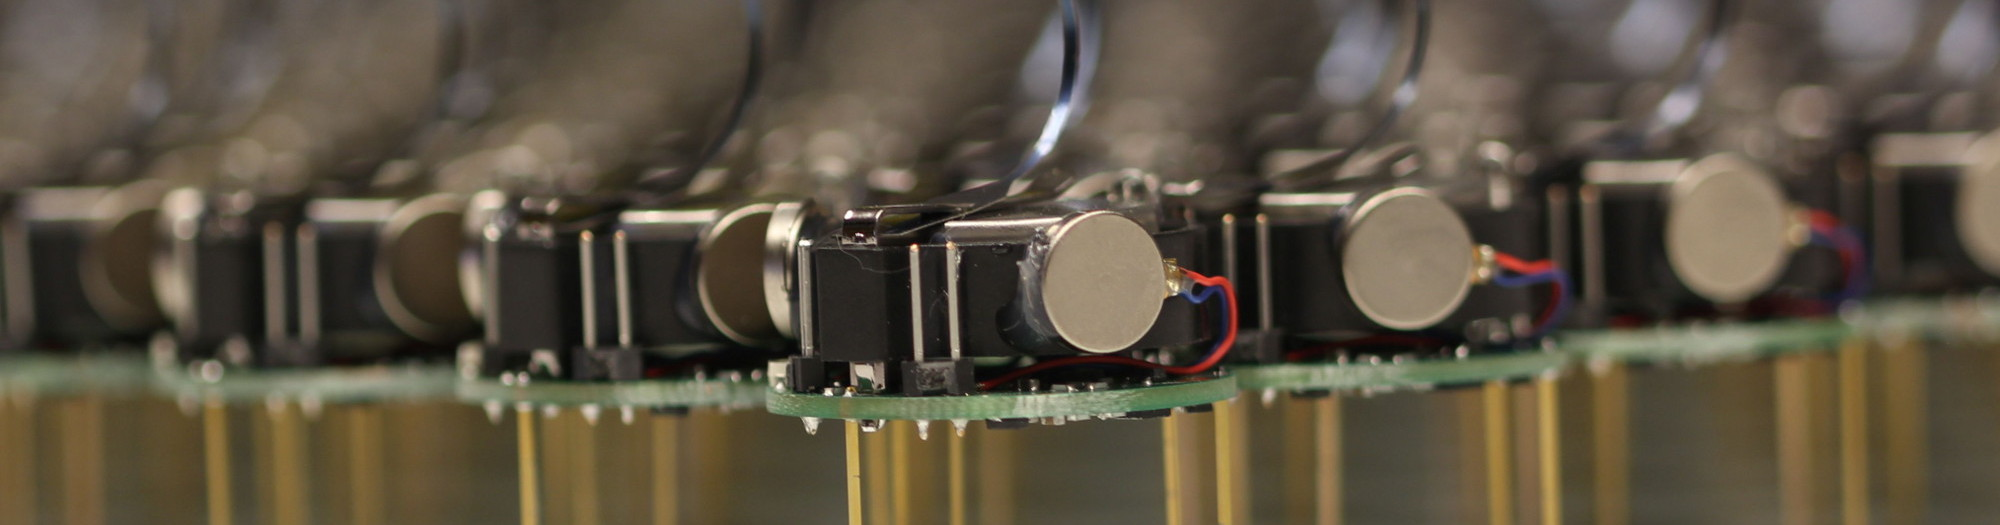
\includegraphics[width=\textwidth,right]{images/kilobots}
        \end{column}%
        \begin{column}{0.25\textwidth}%
            \caption{Kilobots, a common swarm robotics platform \scriptsize{\cite{ssr_lab_harvard_university_swarm2.jpg_????}}}
        \end{column}%
    \end{columns}
\end{figure}

\end{frame}

\begin{frame}{Background}
	\begin{figure}
		\begin{center}
		\includemedia[width=\linewidth,height=0.6\textwidth, flashvars={scaleMode=zoom}]{}{http://www.youtube.com/v/c7kiPri9ZFo?rel=0&amp;showinfo=0}
		\end{center}
		\caption{\href{http://www.youtube.com/v/c7kiPri9ZFo?rel=0&amp;showinfo=0}{Video clip of pheromone deposit and response by foraging ants}}
	\end{figure}
\end{frame}

\begin{frame}{System of Ordinary Differential Equations: Single Ant}

\begin{columns}[T,onlytextwidth]
    \column{0.45\textwidth}
     \alert{effect of pheromone:}
\begin{itemize}
	%\item ant integrates pheromone concentration over ``L'' and ``R'' quarter-circular regions
    \item ant accelerates perpendicular to its orientation
    \item magnitude of acceleration is proportional to the difference in concentration of pheromone over the ``L'' and ``R'' regions
\end{itemize}

	\column{0.1\textwidth}
    \column{0.45\textwidth}

      \begin{align*}
\frac{d}{dt} \begin{pmatrix}\vec{x}\\\vec{v}\end{pmatrix} = \begin{pmatrix}\hdots\\ \hat{\vec{v}}_{\perp}(L - R)\end{pmatrix}
\end{align*}
 \begin{figure}
    	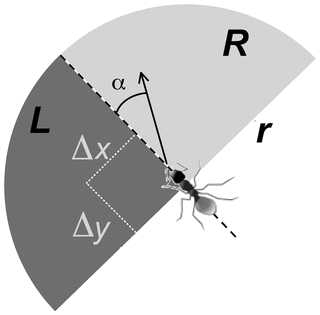
\includegraphics[height=3cm]{images/l_r_regions}
        \caption{Regions of ant sensitivity to pheromone \scriptsize{\cite{perna_individual_2012}}}
    \end{figure}

  \end{columns}
\end{frame}

\begin{frame}{Results (preliminary): Quickest Center-to-Center Path}
\begin{figure}
\begin{columns}[T,onlytextwidth]
\column{0.5\textwidth}
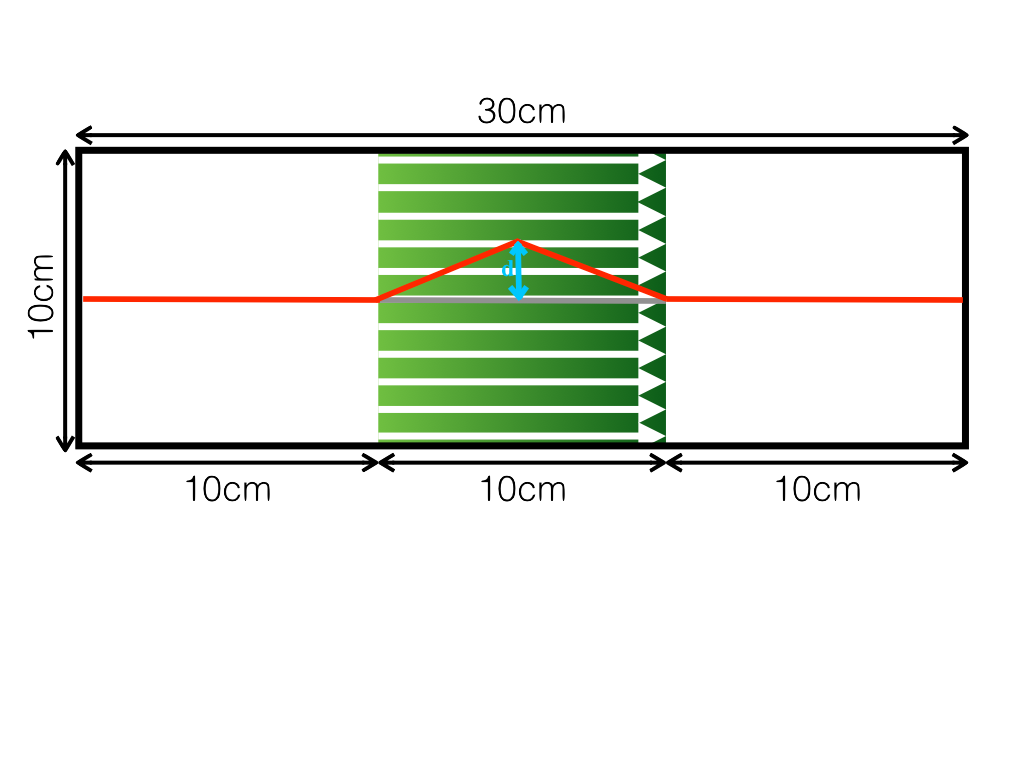
\includegraphics[width=\textwidth]{images/optimal_cen_cen_schematic}
\column{0.5\textwidth}
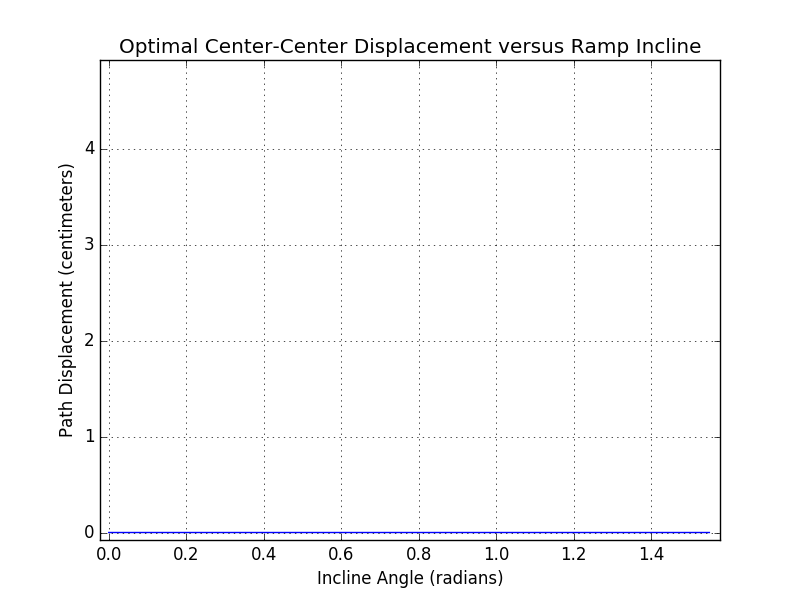
\includegraphics[width=\textwidth]{images/optimal_center_center}
\end{columns}
\caption{Plot of optimal displacement for quickest center-to-center path with schematic showing displacement.}
\end{figure}
\end{frame}

\begin{frame}{Results (preliminary): Quickest Corner-to-Corner Path}
\begin{figure}
\begin{columns}[T,onlytextwidth]
\column{0.5\textwidth}
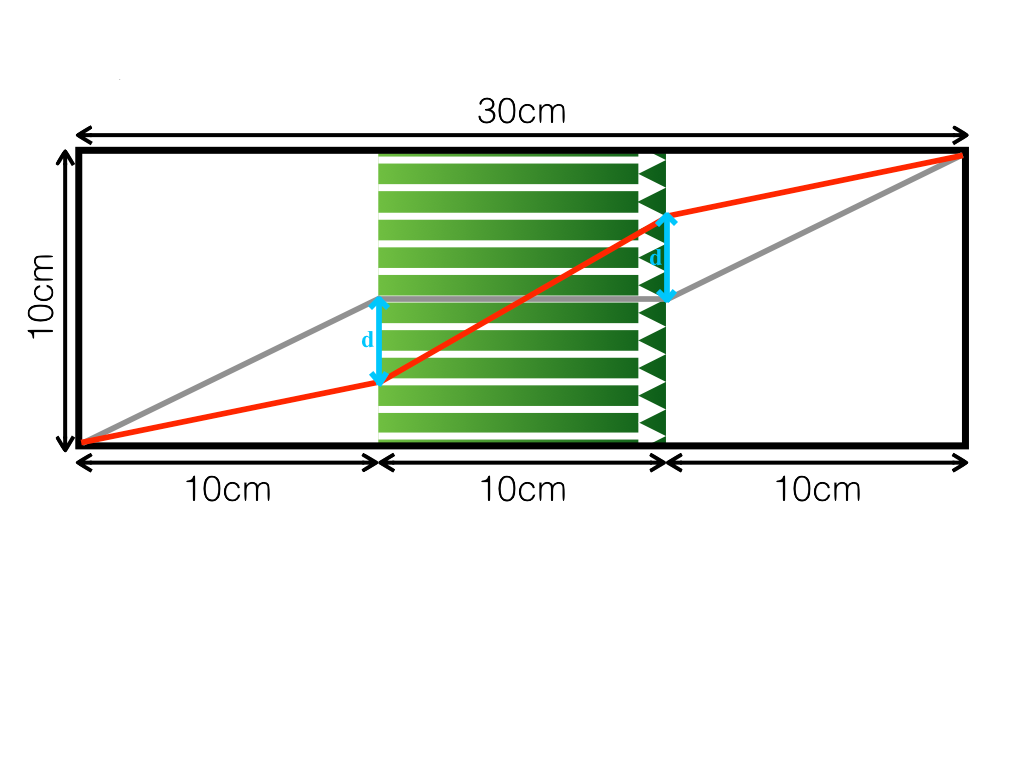
\includegraphics[width=\textwidth]{images/optimal_cor_cor_schematic}
\column{0.5\textwidth}
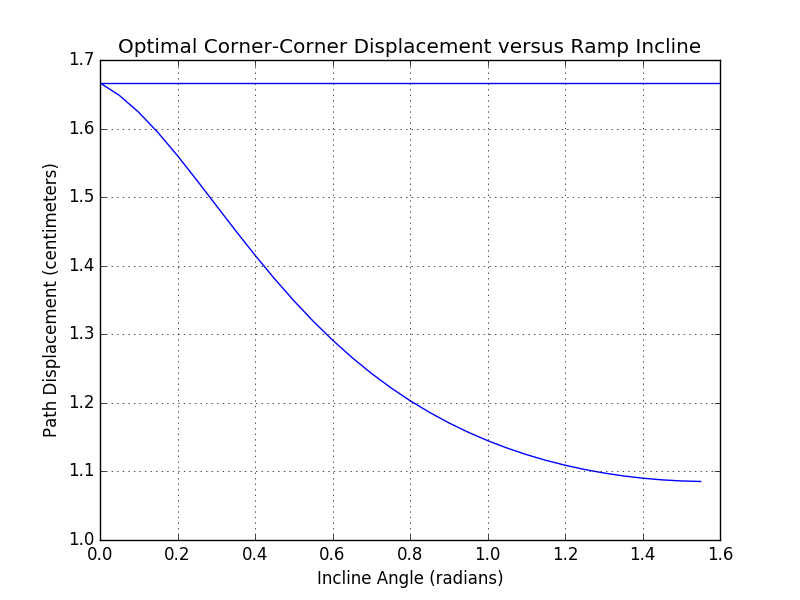
\includegraphics[width=\textwidth]{images/optimal_corner_corner}
\end{columns}
\caption{Plot of optimal displacement for quickest corner-to-corner path with schematic showing displacement.}
\end{figure}
\end{frame}

\begin{frame}{Results (preliminary): Path Shape}
\begin{figure}
\begin{columns}[T,onlytextwidth]
\column{0.33\textwidth}
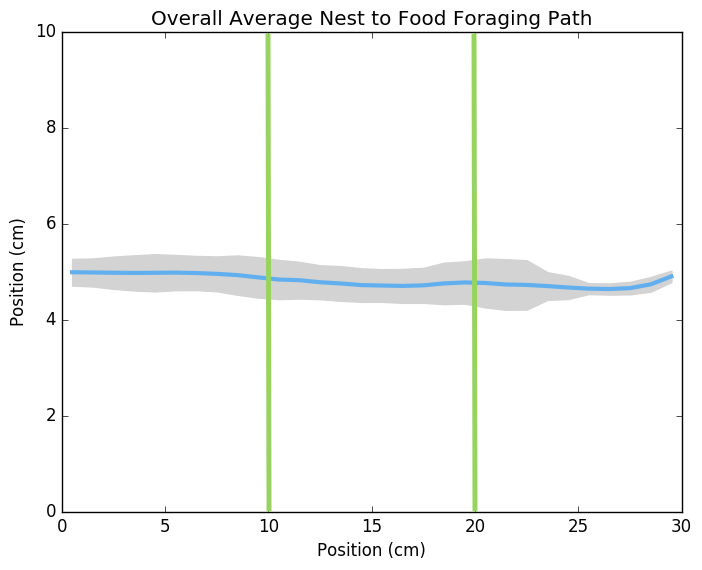
\includegraphics[width=\textwidth]{results/center-to-center-average_path_negpidiv3.png}
\column{0.005\textwidth}
\column{0.33\textwidth}
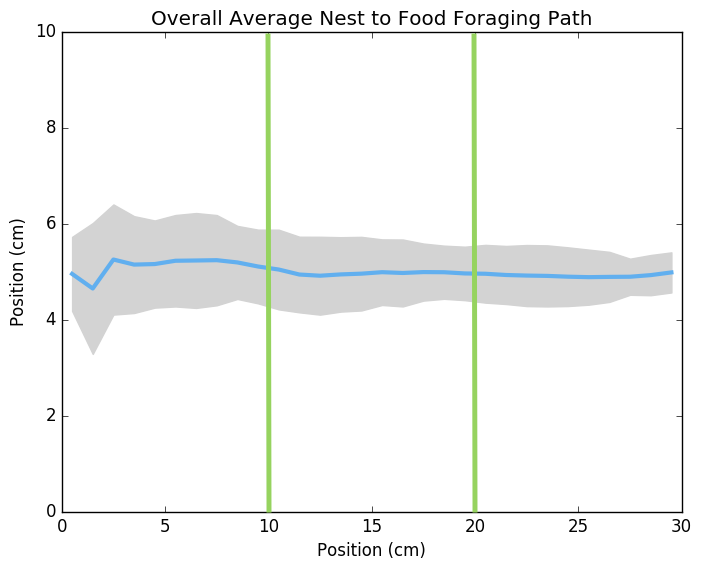
\includegraphics[width=\textwidth]{results/center-to-center-average_path_0.png}
\column{0.005\textwidth}
\column{0.33\textwidth}
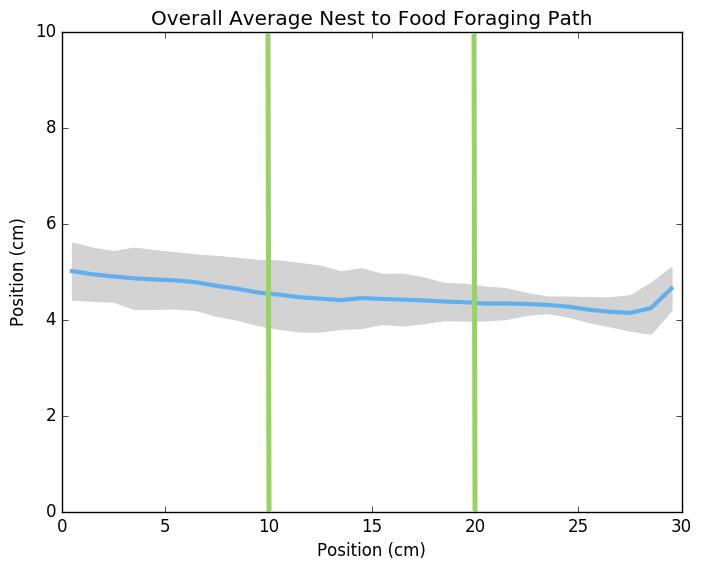
\includegraphics[width=\textwidth]{results/center-to-center-average_path_pidiv3.png}
\end{columns}
\caption{Comparison of overall average nest to food foraging path for, left to right, $-\pi/3$, $0$, and $\pi/3$ radian inclines.}
\end{figure}
\end{frame}

\begin{frame}{Results (preliminary): Path Length}
\begin{figure}
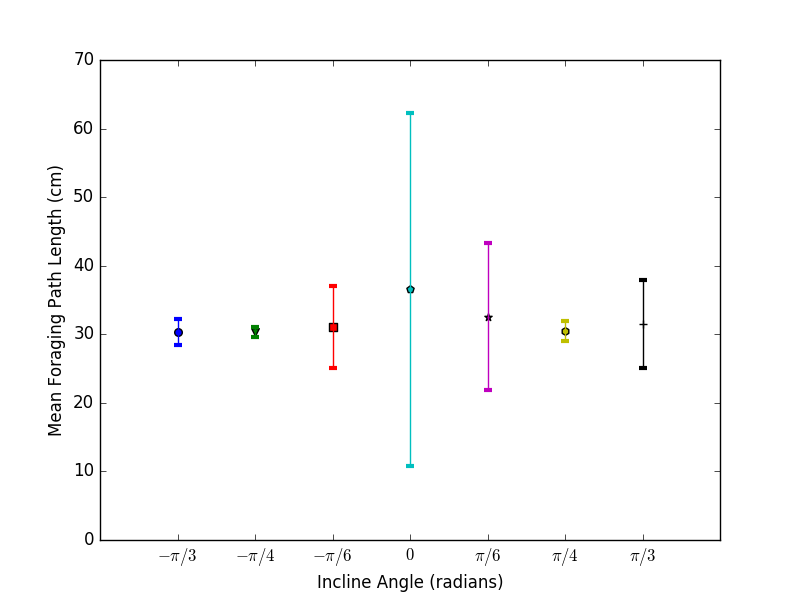
\includegraphics[width=0.8\textwidth]{results/center-to-centermeanforagingpathlength.png}
\caption{Comparison of path lengths over incline angles for center-to-center trials}
\end{figure}
\end{frame}

\begin{frame}{Results (preliminary): Path Smoothness}
\begin{figure}
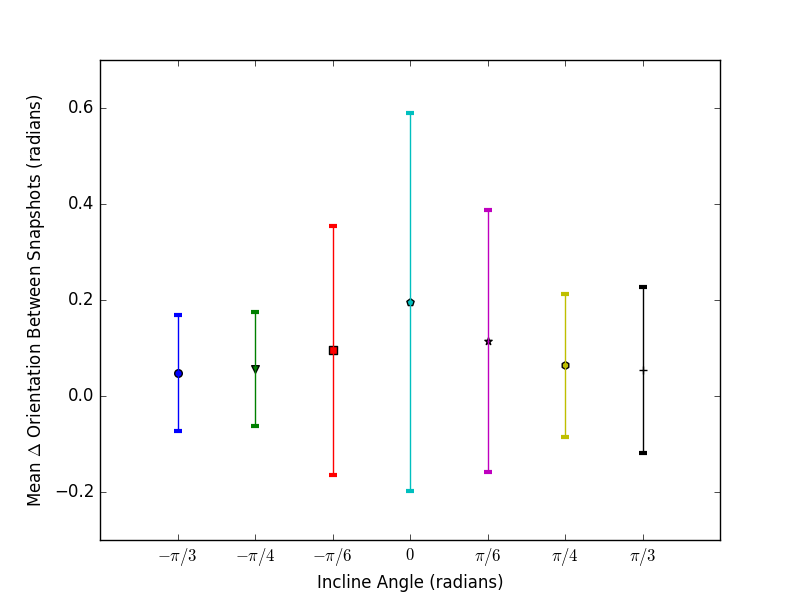
\includegraphics[width=0.8\textwidth]{results/center-to-center_meandeltaorientationbetweensnapshots.png}
\caption{Comparison of changes in heading between shapshots over incline angles for center-to-center trials}
\end{figure}
\end{frame}

\begin{frame}{Results (preliminary): Trip Duration}
\begin{figure}
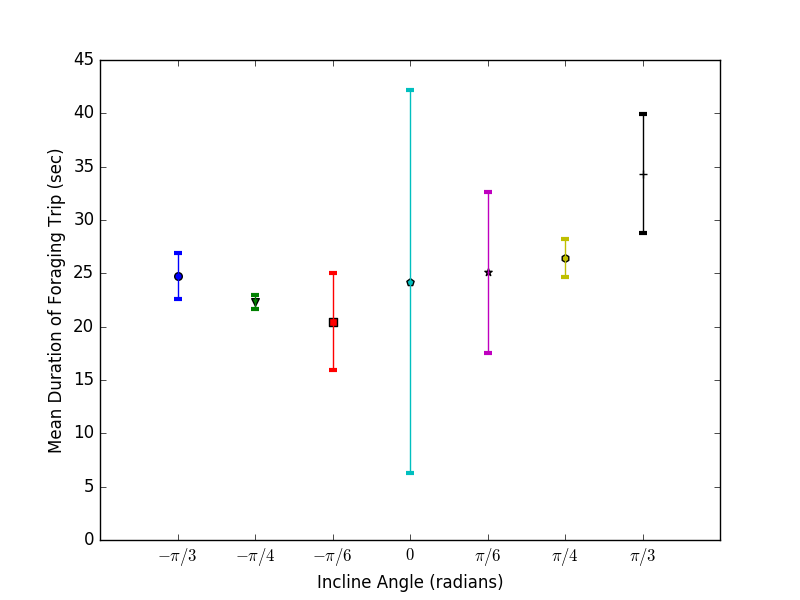
\includegraphics[width=0.8\textwidth]{results/center-to-centermeandurationofforagingtrip.png}
\caption{Comparison of trip durations over incline angles for center-to-center trials}
\end{figure}
\end{frame}

\begin{frame}{Results (preliminary): Orientation Relative to Gradient}
\begin{figure}
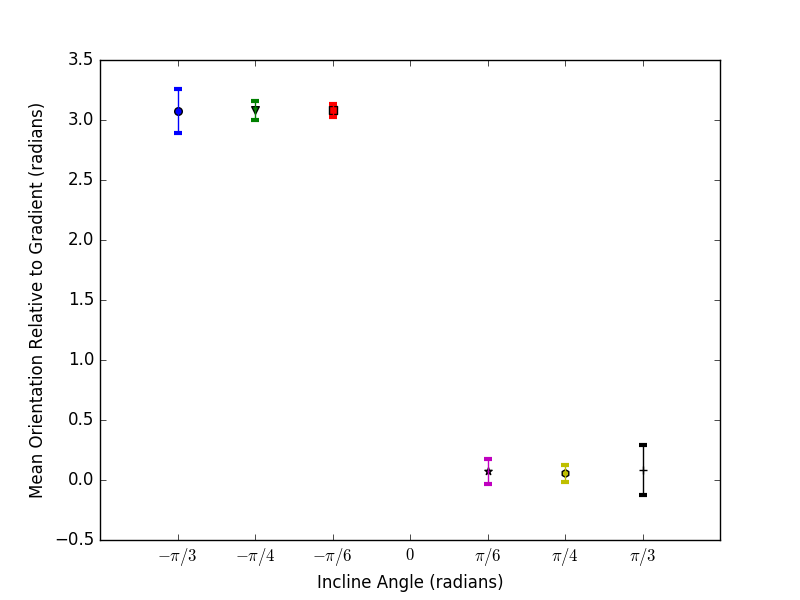
\includegraphics[width=0.8\textwidth]{results/center-to-centermeanorientationrelativetogradient.png}
\caption{Comparison of orientation relative to gradient over incline angles for center-to-center evaporation rates; the straight path is oriented at 0/3.14 radians}
\end{figure}
\end{frame}

\begin{frame}{System of Ordinary Differential Equations: Single Ant}

    	\begin{align*}
			\frac{d}{dt} \begin{pmatrix}\vec{x}\\\vec{v}\end{pmatrix} = \begin{pmatrix}\vec{v}\\ \alpha \hat{\vec{v}}(\xi^2 - \norm{\vec{v}}^2)\end{pmatrix}
		\end{align*}

\alert{self-propulsion: \cite{ryan_model_2016}}
\begin{itemize}
	\item ant accelerates in the direction of its movement if $\norm{\vec{v}}  \xi$
    \item ant accelerates against the direction of its movement if $\norm{\vec{v}} < \xi$
    \item``pushes'' ant towards a fixed speed
    \item $\alpha$ is a constant that governs the magnitude of this effect
\end{itemize}
\end{frame}

\begin{frame}{System of Ordinary Differential Equations: Single Ant}
\begin{align*}
\frac{d}{dt} \begin{pmatrix}\vec{x}\\\vec{v}\end{pmatrix} = \begin{pmatrix}\hdots \\ \beta_{\vec{x}} \frac{\vec{a} - \vec{x}}{\norm{\vec{a} - \vec{x}}} \end{pmatrix}
\end{align*}
\alert{attraction to food/nest:}
\begin{itemize}
	\item ant experiences nest attraction if it is in the returner role
    \item ant experiences food attraction if it is in the forager role
	\item ant accelerates in the direction of the attractor
    \item if multiple attractors are present,
    \begin{itemize}
		\item ant is attracted to nearest food item
        \item ant is attracted to midpoint of nest items
    \end{itemize}
    \item $\beta_{\vec{x}}$ governs the strength of attraction
    \begin{itemize}
    	\item constant for nest attraction
        \item for food attraction, decays exponentially with distance from food
    \end{itemize}
\end{itemize}
\end{frame}

\begin{frame}{System of Ordinary Differential Equations: Single Ant}
\begin{align*}
\frac{d}{dt} \begin{pmatrix}\vec{x}\\\vec{v}\end{pmatrix} = \begin{pmatrix}
\hdots \\
\gamma_{\vec{x}} \hat{\vec{v}}_{\perp} \Big( \hat{\vec{v}}_{\perp} \cdot \frac{\vec{a} - \vec{x}}{\norm{\vec{a} - \vec{x}}} \Big)
\end{pmatrix}  \\
\beta = c_1e^{-c_2\norm{\vec{a} - \vec{x}}}
\end{align*}
\alert{near nest attraction:}
\begin{itemize}
	\item ant experiences attraction with magnitude increasing exponentially with proximity to nest
    \item acceleration is projected onto vector perpendicular to orientation of ant
	\item ensures that ant goes directly to nest if ant is nearby the nest
\end{itemize}
\end{frame}

\begin{frame}{System of Ordinary Differential Equations: Pheromone Deposit}
\begin{align*}
\frac{d}{dt} p = \kappa f(p,s\vec{x}_1,\hdots,\vec{x}_n)
\end{align*}
\alert{pheromone deposit:}
\begin{itemize}
	\item the rate of pheromone deposit is proportional to total speed of ants located at a tile
    \item (ants only deposit pheromone when they move)
    \item let $f(p, \vec{x}_1,\hdots,\vec{x}_n)$ represent a sum of the speeds of of ants associated with the pheromone point $p$
    \item $\kappa$ is a constant governing the magnitude of pheromone deposit
\end{itemize}
\end{frame}

\begin{frame}{Events}
\begin{columns}[T,onlytextwidth]
\column{0.70\textwidth}
\small{
\begin{align*}
t =
\begin{cases}
      0 & \bm{U}_1 < \gamma\frac{b_1 - a_1(\cos^2(\phi)-\sin^2(\phi))[c_1 - \hat{\vec{v}} \cdot \hat{\nabla S}]}{\pi/3} \\
      1 & \text{otherwise}
   \end{cases}
\end{align*}
\begin{align*}
s =
\begin{cases}
      -1 & \bm{U}_2 < \frac{\pi -2 d_2 \cos(\phi) [a_2-2 b_2 \sin(\phi)]}{2 \pi } \\
      1 & \text{otherwise}
   \end{cases}
\end{align*}
}
\column{0.05\textwidth}
\column{0.25\textwidth}
\begin{align*}
\theta_{\operatorname{new}} = \theta_{\operatorname{old}} + \bm{T},\\
\bm{T} \sim \mathcal{N}(\pi/6 \times g,\sigma^2), \\
g = s \times t, \\
\bm{U}_1, \bm{U}_2 \sim \operatorname{unif}(0,1)
\end{align*}
\end{columns}
\alert{random reorientation events on an incline:}
\begin{itemize}
	\item ant reorientation is biased by $-\pi/6$, $0$, or $\pi/6$ radians
	 \item random choices made
     \begin{itemize}
     	\item whether to turn or proceed straight
     	\item if turning, whether to turn left or right
     \end{itemize}
     \item probabilities of these choices determined by
     \begin{itemize}
     	\item $\phi$, ant orientation relative to gradient
        \item $\gamma$, angle of inclination
     \end{itemize}
\end{itemize}
\end{frame}

\begin{frame}{Events}
\alert{random reorientation events on an incline:}
\begin{itemize}
     \item parameters were fit using Matlab's \texttt{lsqcurvefit} and  \scriptsize{\cite{khuong_how_2013}}
\end{itemize}
\begin{figure}
\begin{columns}[T,onlytextwidth]
\column{\textwidth}
\begin{minipage}[]{0.05\textwidth}
~
\end{minipage}%
\begin{minipage}[]{0.315\textwidth}
    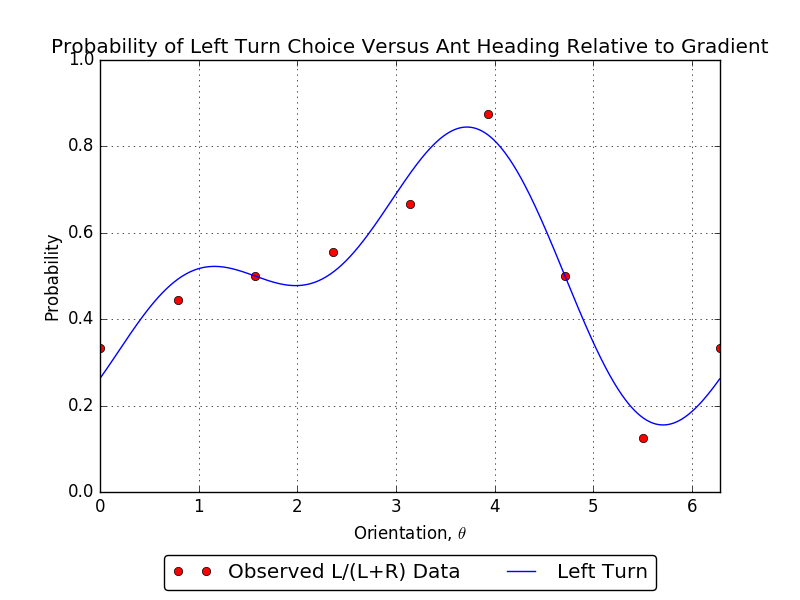
\includegraphics[width=\textwidth]{images/l_choice} \\
    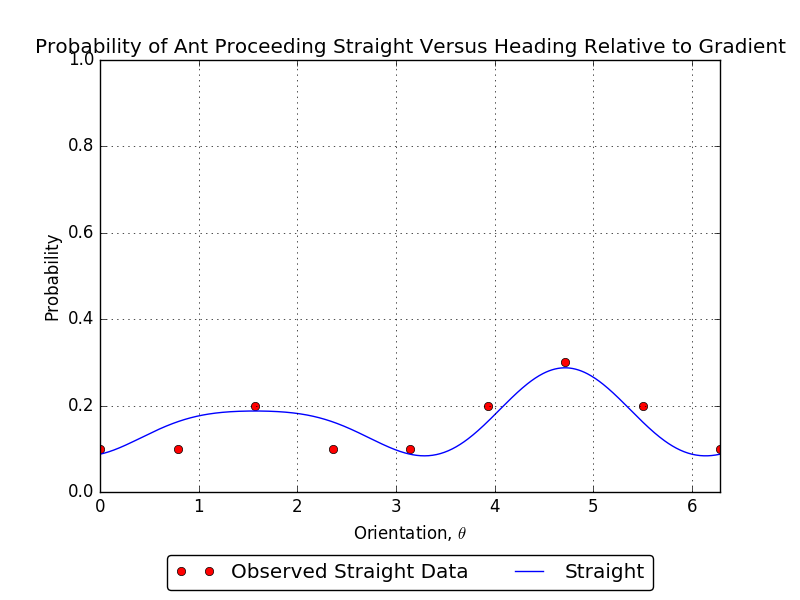
\includegraphics[width = \textwidth]{images/s_choice}
\end{minipage}%
\begin{minipage}[]{0.045\textwidth}
~
\end{minipage}%
\begin{minipage}[]{0.54\textwidth}
    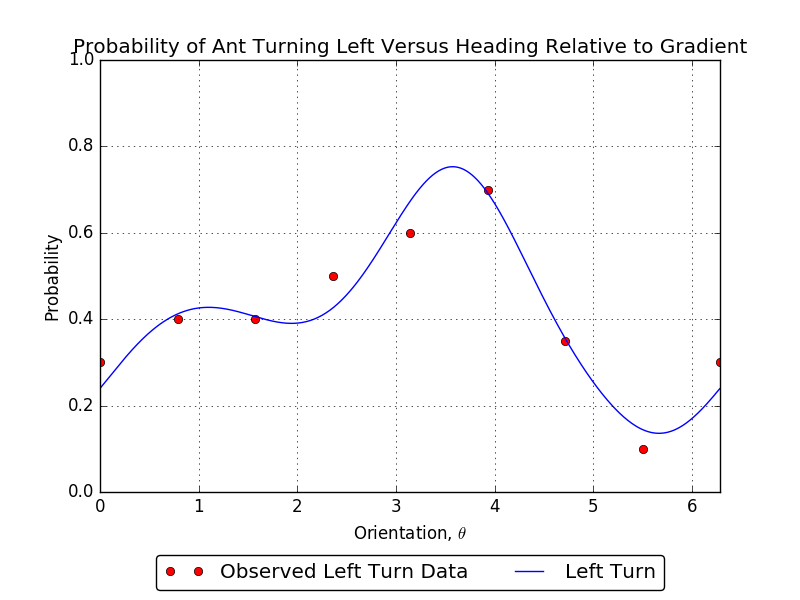
\includegraphics[width = \textwidth]{images/l_result}
\end{minipage}%
\begin{minipage}[]{0.05\textwidth}
~
\end{minipage}%
\end{columns}
\caption{Ant reorientation behavior on an incline ($\gamma = \pi/3$), observed in \cite{khuong_how_2013} versus approximated}
\end{figure}
\end{frame}


\begin{frame}{Numerical Approximation}

\begin{itemize}
	\item deriving an analytic solution is intractable
    \item take a series of small time steps, using each time point to approximate the next
    \item Matlab provides a set of ODE solvers that implement sophisticated algorithms for generating numerical solutions to systems of differential equations
    \item \texttt{ode113} was selected to perform simulations
\end{itemize}
\end{frame}

\begin{frame}{Sensitivity Analysis: Pheromone Evaporation Rate}
	\begin{figure}
	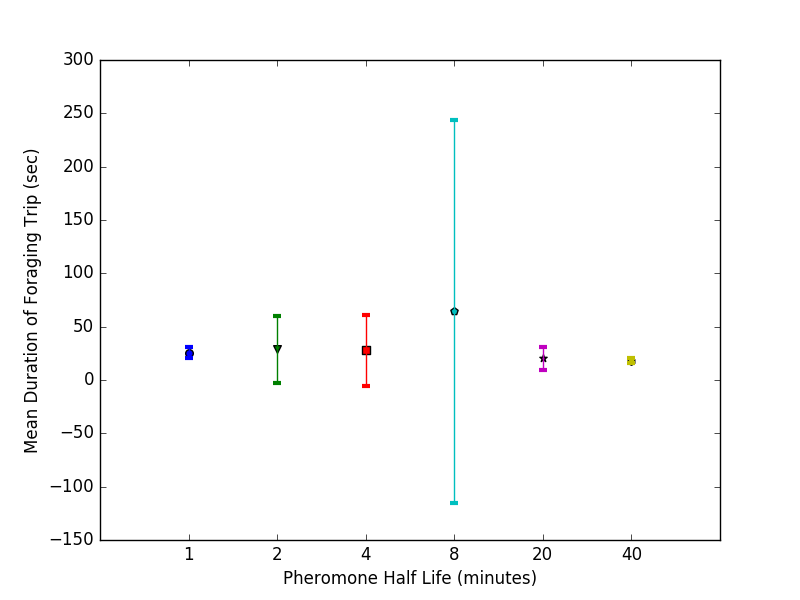
\includegraphics[width=0.8\textwidth]{results/center-to-center-sensitivityanalysis-duration.png}
	\caption{Comparison of durations over pheromone evaporation half lives for center-to-center trials.}
	\end{figure}
\end{frame}

\begin{frame}{Sensitivity Analysis: Pheromone Evaporation Rate}
	\begin{figure}
	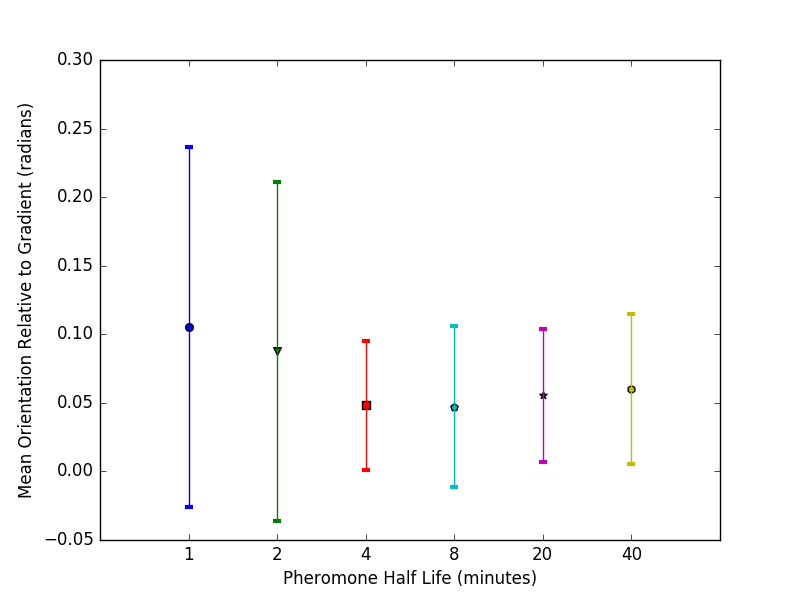
\includegraphics[width=0.8\textwidth]{results/center-to-center-sensitivityanalysis-meanorientation.png}
	\caption{Comparison of orientations relative to gradient over pheromone evaporation half lives for center-to-center trials.}
	\end{figure}
\end{frame}

\begin{frame}{Sensitivity Analysis: Pheromone Evaporation Rate}
	\begin{figure}
	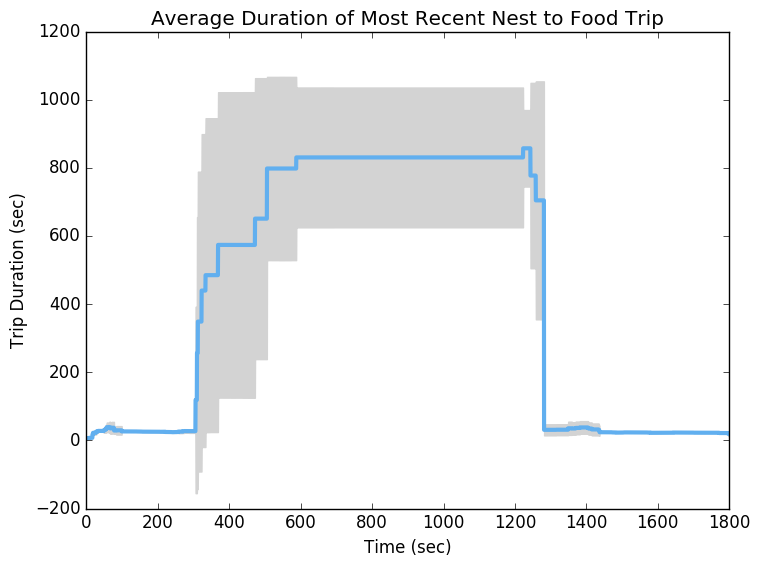
\includegraphics[width=0.8\textwidth]{results/center-to-center-average-trip-duration-8xpheromone.png}
	\caption{Average trip duration over the course of a 30 minute simulation in a center-to-center arena with 8 minute pheromone half life.}
	\end{figure}
\end{frame}

\begin{frame}{Results (preliminary): Path Shape}
\begin{figure}
	\begin{center}
	\includemedia[width=\linewidth,height=0.6\textwidth, flashvars={scaleMode=zoom}]{}{http://www.youtube.com/v/QeSErcTOLbY?rel=0&amp;showinfo=0}
	\end{center}
	\caption{\href{http://www.youtube.com/v/QeSErcTOLbY?rel=0&amp;showinfo=0}{Visualization of path as simulation progresses}}
\end{figure}
\end{frame}

\begin{frame}{Results (preliminary): Path Smoothness}
\begin{figure}
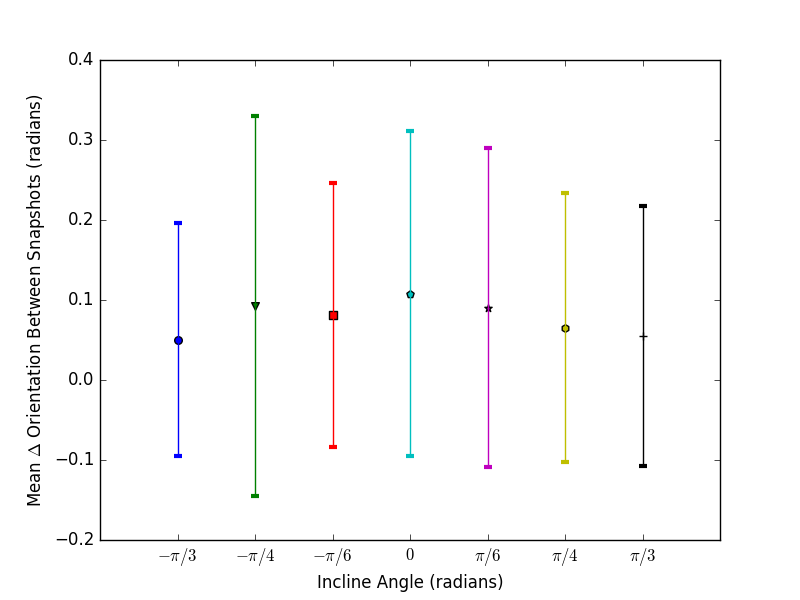
\includegraphics[width=0.8\textwidth]{results/corner-to-corner_meandeltaorientationbetweensnapshots.png}
\caption{Comparison of changes in heading between shapshots over incline angles for corner-to-corner trials}
\end{figure}
\end{frame}

\begin{frame}{Results (preliminary): Orientation Relative to Gradient}
\begin{figure}
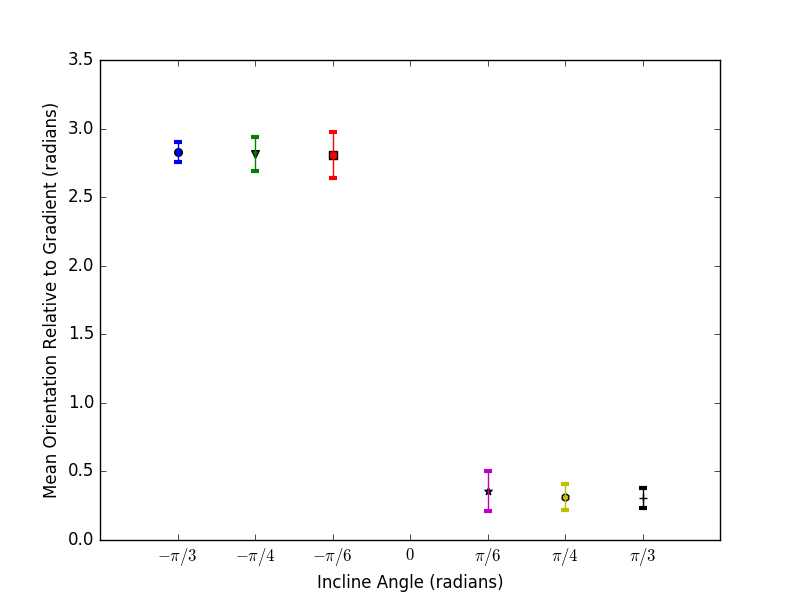
\includegraphics[width=0.8\textwidth]{results/corner-to-cornermeanorientationrelativetogradient.png}
\caption{Comparison of orientation relative to gradient over incline angles for corner-to-corner trials; the straight path is oriented at 2.819/0.321 radians}
\end{figure}
\end{frame}